Consider the first example.

This is the resulting grid after performing the first $3$ updates:

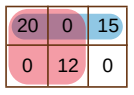
\includegraphics{1.png}

The red rectangle is the rectangle from the first \t{calculate} operation.

The blue rectangle is the rectangle from the second \t{calculate} operation.

After processing $2$ more updates, the grid becomes like in the picture below:

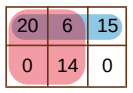
\includegraphics{2.png}

And now the GCD in the red rectangle is $1$, and in the blue rectangle it is equal to $2$.